\chapter{План }

\newpage


\begin{center}
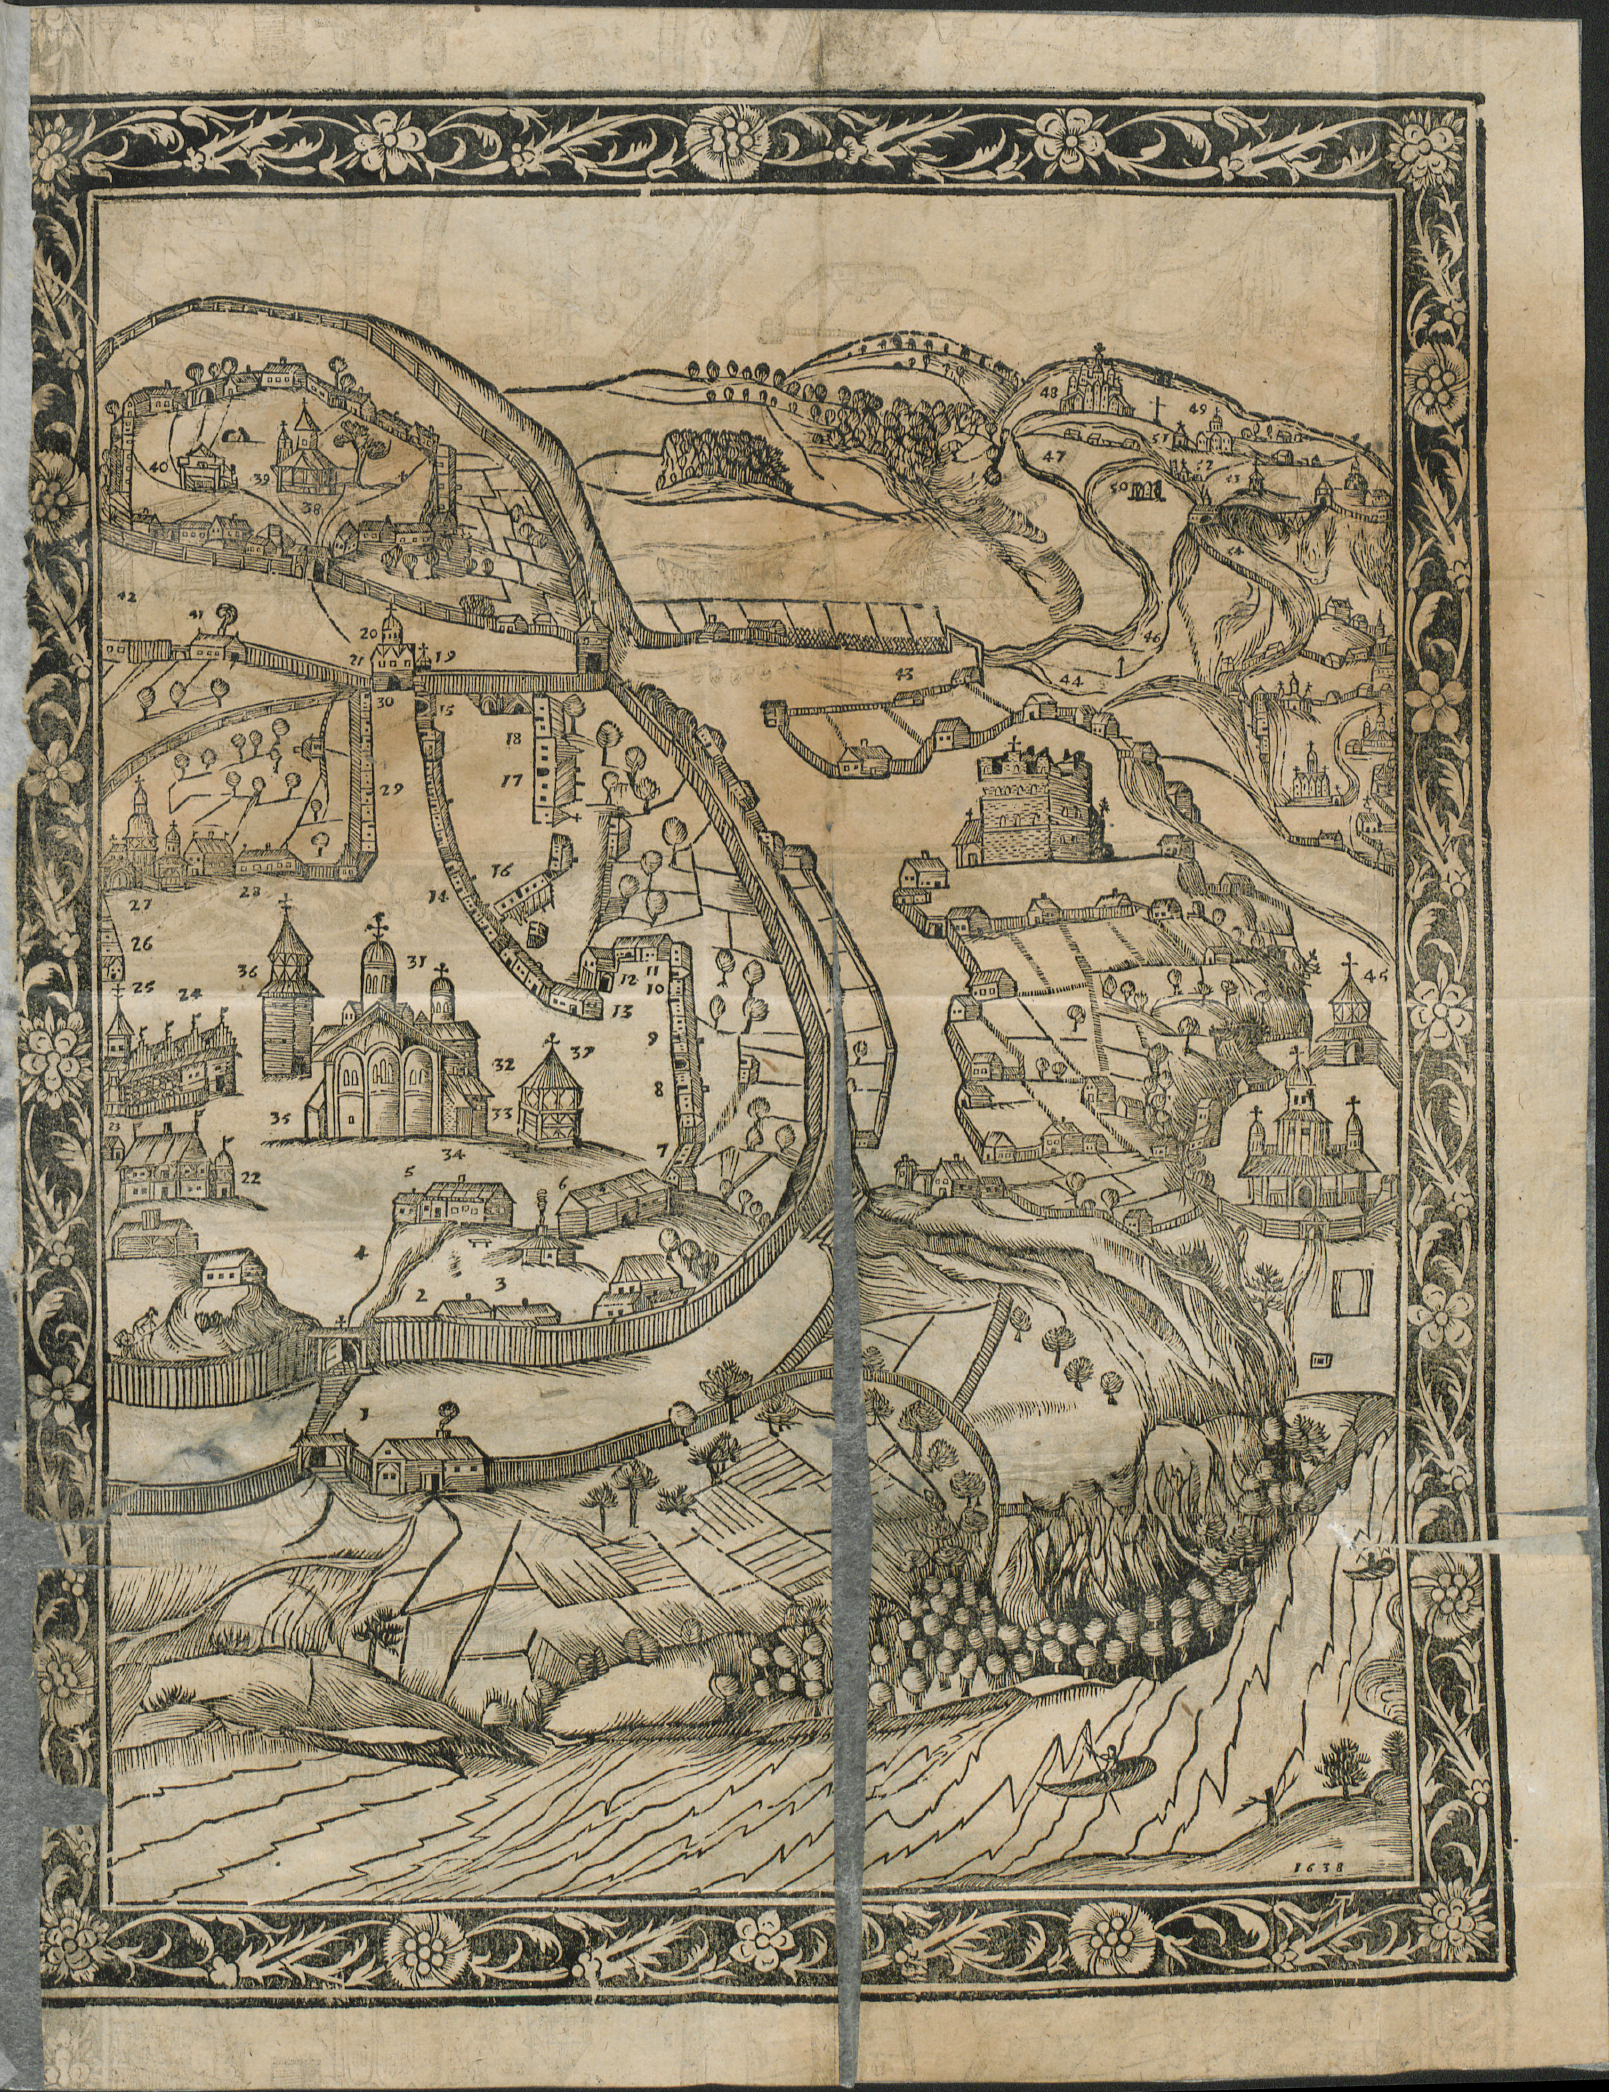
\includegraphics[width=\linewidth]{plan-right/plan-right.png}
\end{center}

\newpage

ЛИСТ 1

1 Cella Ogrodnego brata y ścieżka prześlice do 
Monastyra

1 Келья садовника и тропинка проходящая до монастыря

2 Forta (Sorta?) do samego Cenobium przy ktorey Cella śortarzowa zaraz

2 Forta (Sorta?)  до самого Ксенобиума (монашеское общежитие, киновия ) при которой келья Śortarzowa zaraz

3 Podle tey drugiey Oyca Cella mała

3 Рядом с той вторая отеческая келья малая 

! 4 Obytych po prawej rece dla gory prystra ścieżka do Drukarnie

! 4 По правую руку на гору тропинка к типографии

! 5 Drukarnia na teyże rowninie na ktorey wysłset Monastyr

! 5 Типография на той же равнине, где расположен монастырь

! 6 Piekarnia z spizarniami y wysłsetkim co do nieynależy

! 6 Пекарня с кладовыми и всем, что к ней относится 

! 7 Cella nabożnego brata ktory Piekarnie dogląda

! 7 Келья набожного брата, который заведует пекарней

! 8 Cell starych wrszo cztery

! 8 Четыре старых кельи

9 Cella Zakonnika Polatnego

9 Келья Zakonnika Polatnego 

! 10 Dwie celle iedno/iedna przeciwko drugiey

! 10 Две кельи одна напротив другой

11 Cella od tych coś trochą w sad odemintona

11 Келья тех, что немного в саду

12 Przeciwko tych rzemieslnikom iedne drugie Zakonnicze mieszkanie

12 Напротив их ремесленникам другая келья зальниц

13 Cella wtyle ich przysloyna y spokoyma

13 Келья, прячущая их и успокаивающая

! 14 Od tey mciaz aż do wrot Infirmariey nabożnych Oyców y braci różnych Cell osmaście

! 14 От того места и до ворот Инфирмарии (больницы, лазарета) набожных отцов и братьев различных келий восемнадцать.

15 Wrota do ?osokomiey

15 Ворота в ?osokomiey

! 16 Cell dwie, iedna przeciwko drugiey nabożne Oyców Infirmariey

! 16 Две кельи, одна против друг другой, набожных отцов Инфирмарии

! 17 Sama Infirmaria albo Słowieńska Bolnica gdzie nabożni bracia chorzy opatrzenie przysloney maią miec Cerkiewka przy niey

! 17 Сама Инфирмария или Славянская больница, где набожные братья больные присмотр и утешение имеют, при ней маленькая церковь

18 Cella iedna y komory dla domowych potrzeb schowania przytknione do palow Monastyra wielkie

18 Одна келья и коморы для домашних нужд при главном дворце монастыря

19 Dzwonnica tey ?osocomiey przy Certet murowana y w ?osocomiey przystosione

19 Колокольня этой Косодемии при каменной церкви

ЛИСТ 2



! 20 Sama Certiew Świętey Troyce, czym była stawnęła kośtem, trocha niżey wypisze.

! 20 Церковь Святой Троицы, которой она была построена, немного ниже описана.

! 21 Brama na ktorey ta Certiew stoi.

! 21 Ворота, на которых стоит эта церковь.

! 22 Polewey zaś dla gości dom wysoki na gorze wystawiony.

! 22 Левевее, высокий гостевой дом для гостей на горе поставлен.

! 23 Bibliotheka kiag Cerkiewnych Ruskich, y Sławianskich.

! 23 Библиотека церковных книг русских, и славянских.

! 24 Refektarz niemaly Cerkiew ciepła przy nim, zalozenia ss. Apostołów Piotra y Pawła.

! 24 Трапезная немалая, при ней теплая церковь, заложенная в честь апостолов Петра и Павла


! 25 Wrota do kuchni Bratniey y Archimandryczej y te same kuchnie.

! 25 Ворота к кухне братской и архимандритской и собственно кухни.


! 26 Cell trzy dla sług Archimandryczych.

! 26 Три кельи для слуг архимандрита.

! 27 Pokoie Opactstie.

! 27 Покои аббатские.

! 28 Pod tymże wirzchem Apoteka Monastyrska.

! 28 Под той же крышей Аптека Монастырская.

29 ?owó wysławionych Cell pod iednym nakryciem, dla nabożnych Oyców y braci, iedenascie.

29 ? славных Келий под одной крышей, для набожных отцов и братьев, всего одиннадцать.

! 30 Cella Janitorowa w bramie murowaney z przysionkiem.

! 30 Келья привратника в каменных воротах с крыльцом.

! 31 W pośrodku tak rosporzadzone o Monastyra Cerkiew Wniebowziecia Przeczystey Bogarodzice, tym kształtem stoi, od togo by poczatekswe wysławienia wzięła.

wkatalogu dobodzieiow Claustrinostri opowie sie.

! 31 В середине монастыря расположена церковь Успения Пресвятой Богородицы, прославившая монастырь.

32 Kaplica ss. mm. Panow Jelcow.

32 Каплица святых мучеников Panow Jelcow.

! 33 Kaplica Świętych trzech Cerkiewnych Doktorow Bazylego wielkiego, Hrehoria Theologa, Jana Złotoustego.

! 33 Каплица Святых трех церковных докторов: Василия Великого, Григория Богослова, Иоанна Златоуста.

! 34 Kaplica ss. Jana Bogosłowa.

! 34 Каплица Святого Иоанна Богослова.

35 Kaplica ss. Archidiakona Stephana, Kiazat Jch MM. Korecsich. W tej Ś. Cerkiewi iak by wiele 
bylo ciat błogosławionych Bozych, iat wiele Ksiązecych, Getmanskich, Monastyrskich, Reczypospol:. Dignitarzow, Panow, y osob Przelozonych, Grobow, ich Epitaphia, ktore z roskazania z Stareshego mego, wedle starych nieco przydawszy, na mieczna pamiatke ponowitem: lubo nie wshystkie (dlaraciey w Parenefim po Nagroblash polozoney) iasnie draza. Niedaleko

35 Каплица святого архидиакона Стефана, монастырь их мучеников братьев. В этой церкви также много эпитафий для благословенных братьев, много актов и святых книг монастырских рукописей. Дисциплинарий под господами и предками. Оба эпитафия из этого, из учета старого письма, и нового, ничего не добавили и ничего не убавили.


ЛИСТ 3

pamiętać ponowiłem: lubo nie wszystkie (dla racyey w Paraneśim po Nagrobłach położoney) iasnie widza. Niedaleko


! 36. Dzwonnica iedna wysoka.

! 36. Колокольня одна высокая.

37. Druga zas dla wielkiego cieżaru, ktory na niey iest podnieśiony, to iest Dzwon wielki od autora swego Bałtyka rzeczony, nizsza. Z Cerkwi tedy iść po mie dzy te obiednie do bramy, ktora y na ktorey Cerkiew Świętey Troyce Książę Mikołay Światosha Dawidicz zalozyl, y przyney dla chorych y nie dołężnych zakonników Infirmaria, o ktorey wyżey wspomniałem, fundował, osoblibwego Nosokoma postanowil: ten teraz od Achimandryty Pieczarskiego dependet.
Ta brama wyniść na Miasteczko w ktorym wiele płomnych sirot, wdow ,zebrakov, tak wlasnie przy Cerkwi Ś. Pieczarskiey oszekiwaiac zmiłowania Pańskiego, Ieza: iako było przy oney Sadzawce, ktora Anyoł Pański zstepuiac co rokzamecat.

37. Другая, как для большого веса, который на неё поднят, то есть Большой колокол, автором своим Балтыком названный, ниже. Из Церкви идти по мне эти три обе одни ворота, которые на и которой Церковь Святой Троицы князь Николай Святский навечно основал, и при ней для больных и слабых монахов Инфирмария, о которой выше упоминал, основал, любимую Церковь Святую, и эта теперь на Земельских Печарского зависит. Эти ворота выйти в Город, в котором много пламенных сирот и вдов собрано так же именно при Церкви Святой Печарской, ожидающей милости Господней есть, как было при той Сашавец, которую Ангел Господний спускается до замета.


38. W tym iest Klasztor PatiensSi wiele Miesz. Moie wodzianie Slachcianie i inny rozmaitego stanu w pochody śmiercobliwych zakonników ze zamieniu mający. W tym iako ona Prorokini Anna córka Phanuelowa z potolenia Aser przy Cerkwi 283 lat przemięszkać, iakaienta swoie w pośtach i modłach, pracy y w świątyniach częstey iako tym pilnie y im wiecey onych w pamięci iako dziesięć onych Panien rozdzielenie, by snadź dolu zamiłowania Pańskiego iest, iako było przy oney Saszawec, ktora Anyoł Pański iestępuiać do zamiecał.

38. В этом монастырь Патиенси много жителей. Мои водяне шляхтичи и другие различного статуса в шествиях смертельных монахов за обмен имеют. В этом как та Пророчица Анна, дочь Фануэля, из рода Асера, при Церкви 283 лет жила, которая свои в постах и молитвах, труде и в храмах частой, как тем усердно и более они в памяти как десять тех Дев разделение, чтобы возможно долу милости Господней есть, как было при той Сашавец, которую Ангел Господний спускается до замета.




СТРАНИЦА 4

39 W posrodku tegoż Monastyra Cerkiew.

39 В середине этого монастыря церковь.


40 Ulice Isakowego Studnia.

40 Улица Исаакова колодца.


41 Naprzeciwko tegoż Monastyra Pańskiego Dom gościnny dla Słatonney Braciéy y Pielgrzymow.

41 Напротив этого монастыря Господский гостевой дом для благородных братьев и паломников.


42 Ku Południe przez Miasto droga tu Lybedzi.

42 На юг через город дорога к Лыбеди.

43 Miedzy Zapadem y Północą droga idziemy przez Tatarskie Spaliki, to iest mimo Cerkiew Przemienienia Pańskiego, tą ś Włodzimierz murował. lecz iey ściany zaledwie teraz stoia, rumy ziemie okryły y przez pośde do teyże Światnice Pańskiey maleiąca.

43 Между западом и севером дорога идет через татарские развалины, это мимо церкви Преображения Господня, которую Владимир построил. Но её стены едва стоят сейчас, руины покрыты землёй, и через них идешь к той же Святыне Господней, уменьшающейся.


44 Po teyże prawej stronie przeszedłszy nieco drożkiey droga do Monastyra ś. Mikołaiá Pustynnego. Sam Klasztor tego ś. Archiereia.

44 По той же правой стороне, пройдя немного дальше, дорога к монастырю Святого Николая Пустынного. Сам монастырь этого Святого Архиепископа.

45 Po teyże rece daley trochę drożką do Przewozu na Dnieprze.

45 По той же руке дальше немного дорогой к переправе на Днепре.

46 Minąwszy te iść prosto przez odd do wałów wielkich, w tych

46 Пройдя это, идти прямо через вал великий, в этих

47 Cerkiew Świętey Sophiey iádo w własnym Cnym, w swoim tytro wtrąg aż do bramy Mięysciey przciąga się iá znacznie poprawiona y w nowo poczęta.

47 Церковь Святой Софии, в собственном благородном, в своём титуле простирается до городских ворот, значительно улучшена и вновь начата.


48 Cerkiew ś. Archinyola Micháła, y Monastyra.

Церковь Святого Архангела Михаила и монастырь.

СТРАНИЦА 5


50 Certwie Św. Theodora Tyrona tylko śliczny Stoia, ktorey tak iako y o drugich Certwiy ŚŚ. Aliom ślich ruinach rzec 3 Poeta moge: Quaeq; prius Sanctos cogebat curia patres, Serpentum facta est alituumq; domus, Plenaq; tot passim generosis atria ceris, Ipsa sua tandem subruta mole iacent. Calcanturq; olim sacris onerata tropheis Limina, distractos \& tegit herba Deos. Tot decora artificumq; manus, tot nota sepulchra, Totq; pios cineres vna ruina premit.

To iest: Do ktorych z Ispym Xięźęta Senatem wchodzili Cerkwie te teraz z pałacem węźę napełnili. Pełne Świętych przedtym ciał Światnice wpadły, Jedne popiołem, drugie rumami siadły. Święte progi Poganin chodzić depe smiele Niedba iż chwałsem Świętych Ciały starata wiele. Miśerne dech mnie prace, groby wynisione. Jednym upadłem cięźko lecą przypylone.

50 Церковь Святого Феодора Тирона стоит красиво, которая, как и другие церкви, могла быть описана поэтом: Которые прежде святых отцов к консистории вели, Теперь стали домом для змей и птиц, Полные величественных залов, теперь под обломками лежат. Когда-то священные пороги, теперь покрыты травой. Множество искусных рук, множество известных гробниц, И благочестивых пеплов в одну руину собрались.

Это значит: Куда раньше князья и сенаторы входили Церкви теперь заполнили змеи. Святые помещения, раньше полные тел святых, развалились. Одни покрылись пеплом, другие разрушены. Святые пороги теперь посещаются паганами, Не заботясь о святости тел. Много труда ушло на поднятые гробницы, Теперь всё это пеплом покрыто.

51 Certkiew Św. Basilego na samy przod murowana od Wielkiego Włodzimierza.

51 Церковь Святого Василия, построенная великим Владимиром.

52 Certkiew Naswietszey Panny Dziesiecinna.

52 Церковь Пресвятой Девы Десятинная.

53 Certkiew Św. Simeona nad samym Kiiowem a drugie mogiłami leżą przed obo nad więty przywislone.

53 Церковь Святого Симеона рядом с Киевом, а другие могилами лежат перед обоими [церквяим Симеона и Десятинной] 


54 "Z tych Brama: mimo Zamek na wosstłey gorze erigowany w dol sie spuscić do oplotanego Zitowa; poniewaz starego terasnieysz y zaledwie imienia godzien: w tamtym Cerkwi było wiecey niz trzysta murowanych, sto drewnianych: w tym zaledwie wsystkich trzynascie: wtamty fly dziesieciny do Cerkwi Taswiéltey Panny, o Dziesiecin Dziesiecinney rzeczoney ze wsystkiey Rusi na ten czas, a teraz"


54 "Из этих ворот: мимо Замка на высокой горе спуститься вниз к оплетённому Житову; потому что старого нынешнего едва ли имени достойного: в том церкови было более трехсот каменных, сто деревянных: в этом едва ли всех тринадцать: в том десятину к церкви Пресвятой Девы, о Десятине Десятинной, сказанной со всей Руси на то время, а теперь"

